
%(BEGIN_QUESTION)
% Copyright 2006, Tony R. Kuphaldt, released under the Creative Commons Attribution License (v 1.0)
% This means you may do almost anything with this work of mine, so long as you give me proper credit

Answer the following questions about this analog proportional controller circuit:

$$\includegraphics[width=15.5cm]{i01494x01.eps}$$

\begin{itemize}
\item{} How is the proportional band setting adjusted?
\vskip 10pt
\item{} How is the bias setting adjusted?
\vskip 10pt
\item{} Which switch position is for {\it direct} action and which is for {\it reverse} action?
\vskip 10pt
\item{} Calculate the proportional band for this circuit if all $R$ values are precisely equal, and if both potentiometers are set in mid-position.
\end{itemize}

\vfil 

\underbar{file i01494}
\eject
%(END_QUESTION)





%(BEGIN_ANSWER)

This is a graded question -- no answers or hints given!

%(END_ANSWER)





%(BEGIN_NOTES)

We know that {\it proportional band} is related to the {\it gain} of the controller, and therefore whichever potentiometer sets the gain (amplification) of this controller circuit will be the proportional band adjustement.  This can only be the potentiometer found in the feedback network of the final opamp.

\vskip 10pt

We know that {\it bias} is an added quantity to the output ($m$) of a loop controller.  As such, we need to look for any potentiometer in this circuit that biases or offsets the output voltage.  In this case, that potentiometer is the one connected as a voltage divider to the non-inverting input of the final opamp.

\vskip 10pt

{\it Direct action} is defined as the output of a loop controller increasing in response to an increased process variable (PV) input, while {\it reverse action} is defined as the output of a loop controller decreasing in response to an increased process variable (PV) input.  We may determine which switch position is which direction of controller action by performing ``thought experiments'' whereby we imagine the $V_{process}$ signal increasing and then we determine which direction $V_{output}$ changes.  Beginning with the switch position as shown in the diagram, an increasing $V_{process}$ is sensed at the non-inverting input of the first opamp, driving that output voltage upwards.  This rising signal is sensed at the inverting input of the next opamp, driving its output voltage down.  That signal is sensed at the inverting input of the final opamp, driving the $V_{output}$ upwards.  Therefore, the switch position as drawn is for {\it direct action}.

\vskip 10pt

If all $R$ values are equal and both pots are in mid-position, the controller will have an over-all gain of 2 (P.B. = 50\%).  The final (right-hand side) opamp is an inverting amplifier whose gain is 1 with equal input and feedback resistance values in the feedback network.  The other two opamps are configured as noninverting amplifiers (with respect to the PV and SP inputs) having gains of 2 with equal-value resistors in their feedback networks.

%INDEX% Control, proportional: analog electronic controller

%(END_NOTES)


